%!TEX program = xelatex
\documentclass[nobib, nohyper, a4paper,openany]{tufte-book}
\XeTeXinputnormalization=1


\usepackage[babel,german=quotes]{csquotes}
\usepackage{polyglossia}
\setdefaultlanguage[spelling=new,babelshorthands=true]{german}
\setotherlanguage[]{english}
\usepackage[xetex,bookmarks=true,colorlinks=true,linktoc=section,]{hyperref}
\usepackage{booktabs}
\usepackage{amsmath}
% \usepackage{color}
\usepackage{xcolor,listings}
\colorlet{punct}{red!60!black}
\definecolor{background}{HTML}{EEEEEE}
\definecolor{delim}{RGB}{20,105,176}
\colorlet{numb}{magenta!60!black}
\lstset{ %
basicstyle=\normalfont\ttfamily,
numberstyle=\scriptsize,
stepnumber=1,
numbersep=8pt,
backgroundcolor=\color{background},
}

\lstdefinelanguage{json}{
    basicstyle=\normalfont\ttfamily,
    numberstyle=\scriptsize,
    stepnumber=1,
    numbersep=8pt,
    showstringspaces=false,
    breaklines=true,
    backgroundcolor=\color{background},
    literate=
     *{:}{{{\color{punct}{:}}}}{1}
      {,}{{{\color{punct}{,}}}}{1}
      {\{}{{{\color{delim}{\{}}}}{1}
      {\}}{{{\color{delim}{\}}}}}{1}
      {[}{{{\color{delim}{[}}}}{1}
      {]}{{{\color{delim}{]}}}}{1},
}
\usepackage{subcaption}
% tufte fix
\ifxetex
\newcommand{\textls}[2][5]{%
  \begingroup\addfontfeatures{LetterSpace=#1}#2\endgroup
}
\renewcommand{\allcapsspacing}[1]{\textls[15]{#1}}
\renewcommand{\smallcapsspacing}[1]{\textls[10]{#1}}
\renewcommand{\allcaps}[1]{\textls[15]{\MakeTextUppercase{#1}}}
\renewcommand{\smallcaps}[1]{\smallcapsspacing{\scshape\MakeTextLowercase{#1}}}
\renewcommand{\textsc}[1]{\smallcapsspacing{\textsmallcaps{#1}}}

\fi
% --
\makeatletter
\newcommand\chapterauthor[1]{}
\def\@chapterauthor{}
\fancypagestyle{mystyle}{%
\fancyhf{}%
\renewcommand{\chaptermark}[1]{\markboth{##1}{}}%
\fancyhead[LE]{\thepage\quad\smallcaps{\newlinetospace{\leftmark}}}% 
\fancyhead[RO]{\smallcaps{\newlinetospace{\@chapterauthor}}\quad\thepage}%
}
\makeatother


\usepackage{fontspec}
\usepackage[parfill]{parskip}
\setlength{\parindent}{0pt}

% \setromanfont[Mapping=tex-text]{Linux Biolinum}
\setsansfont[Mapping=tex-text]{Gill Sans}
\setmonofont[Mapping=tex-text,Scale=0.8]{Droid Sans Mono}
\newfontfamily{\sym}{FontAwesome}
\newcommand*{\user}{{\sym^^^^f007 \selectfont}}
\newcommand*{\comment}{{\sym^^^^f075 \selectfont}}
\newcommand*{\relto}[2]{\(\text{#1} \mapsto \text{#2}\)}
\newcommand*{\lang}{{\sym^^^^f1ab \selectfont}}
\newcommand*{\ca}[1]{\textcolor{cyan}{#1}}
\newcommand*{\cb}[1]{\textcolor{RedOrange}{#1}}
\newcommand*{\maththree}[1]{\text{#1}_1,\text{#1}_2,\text{#1}_3}
% \newcommand*{\sym}{\fontfamily{FontAwesome}\selectfont}
\usepackage{scrextend}
\addtokomafont{labelinglabel}{\sffamily}

\usepackage{graphicx}
\usepackage[
    % sorting=nyt,
    % style=alphabetic,
    % citestyle=alphabetic,
    % bibstyle=authoryear,
    % % natbib=true,
    style=alphabetic,
    % autocite=footnote,
    backend=biber
    ]{biblatex}
\addbibresource{imi-ic-viscom.bib}



\newcommand{\jc}[1]{\texttt{#1}}
\newsavebox{\titleimage}
\savebox{\titleimage}{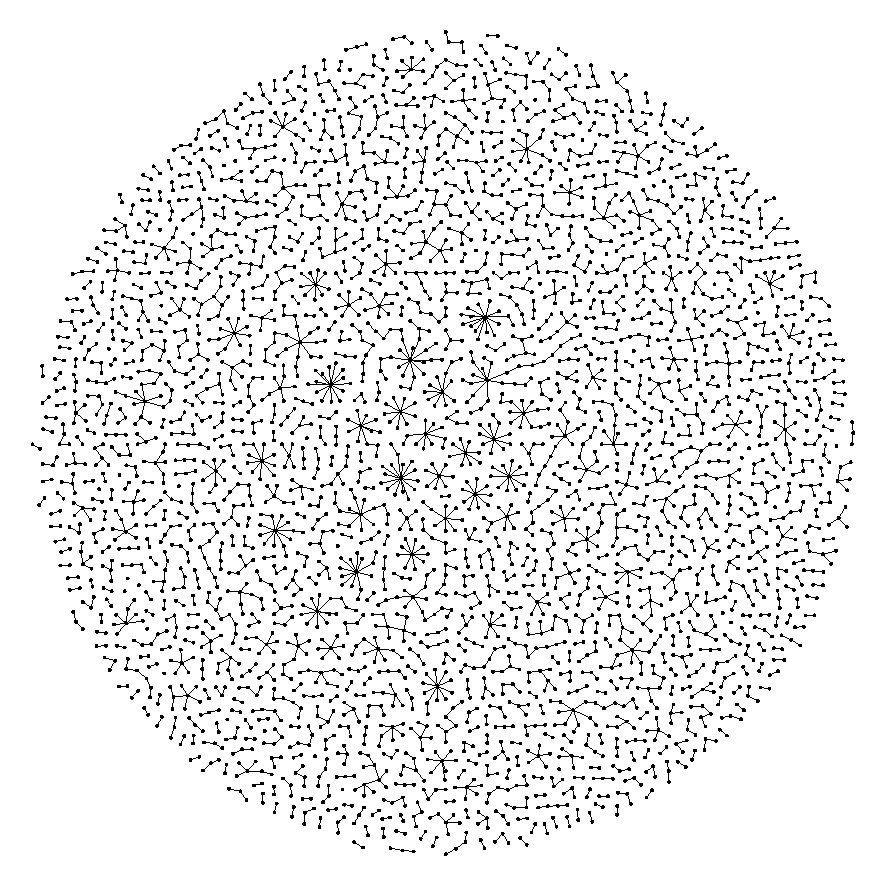
\includegraphics[width=12cm]{figures/comment_graph.pdf}}

% \author{Jakob Schmolling}
\title[IC 2]{
  \vfill
\usebox{\titleimage}\\
\noindent
\huge{Independent Coursework 2}\\
\noindent\Large{Visualisierung von Webforumsdaten}}


\publisher[HTW Berlin]{HTW Berlin / \today}

% \pu
\begin{document}

\maketitle
\tableofcontents
% \section{Einleitung}
% \chapter{Einleitung}



\chapter{Öffentliche Diskussion im Netz}
 
Internetkommentare werden mit zunehmender Bedeutung nicht nur Ort von Debatten, sondern auch öfter Diskursobjekt. 
Die Verbreitung von Textbeiträgen über das Internet in Form von Postings, Kommentaren und Kurznachrichten bildet heute den Grundpfeiler aller \textbf{``Social Media''} Plattformen.
Plattformen wie Facebook, Twitter und Reddit stellen Möglichkeiten für öffentliche Diskurse bereit.
Diese Plattformen haben die Grenzen zwischen Sender und Empfänger aufgeweicht. 
Aber eine textbasierte Kommunikation beeinflusst auch wie wir Kommunikation verstehen, ``the media is the message''.
Eine Kommunikationsform, die vielen Sprechern eine Stimme gibt, ist demokratisch, aber nicht ohne Probleme.
Unternehmen, Gruppierungen und Einzelpersonen ringen um Aufmerksamkeit für ein größeres Sprachrohr. 
 

\subsection{Ziel der Arbeit}
In dieser Arbeit soll es um Social Media Diskussionen gehen. 
Aktuell hat diese Kommunikationsart einen Umfang erreicht, der nicht mehr leicht verständlich ist.
Die Arbeit versucht die Untergruppe der \textbf{öffentlichen, asynchronen und textbasierten Kommunikation zu visualisieren}.
(Also zum Beispiel Foren, Kommentare auf Nachrichtenseiten oder Blogs).
Die Technologie dieser Kommunikation wird im ersten Teil untersucht. 
Eine Kategorisierung unterschiedlicher Kommunikationmodi erfolgt im zweiten Teil.
Für praktischen Teil der Arbeit wurde eine Visualisierung entwickelt basierend auf einer 
Kategorisierung (\nameref{sec:Threaded}) aus dem zweiten Teil.



\section{Entwicklung der Diskussionsplattformen}
Internetnutzer in den 80er und 90er Jahren hatten meist das nötige ``know-how'' 
um Programme wie Bulletin Boards, Usenet und IRC zu nutzen und teilweise auch zu hosten.
Mit dem Aufkommen von HTML wurde das Internet immer einfacher zugänglich.
Software wie phpBB\cite{phpBB2017} erlaubt es jedem mit einem Browser an einer Diskussion teilzunehmen. 

Heute wird das Internet von Social Media Plattformen dominiert.
In den USA sind 67\% der Erwachsenen Facebook-Nutzer und 44\% nutzen die Seite auch um sich über Nachrichten
\marginnote{Nachrichten im Sinne von \emph{news}, nicht \emph{messages}}
zu informeren\cite{GottfriedNewsUseSocial2016}. 
Zusammen mit anderen Plattformen (Twitter, reddit, Tumblr)
sind es für Millionen Menschen möglich an öffentlichen Debatten teilzunehmen.

\subsection{Motivation}
Warum wird dieses Feature überhaupt genutzt? 
Was sind die Gründe im auf Nachrichtenseiten zu kommentieren? 
Eine Umfrage über die Motivation von Nutzer, die auf Newsseiten kommentieren\cite{StroudCommentSectionSurvey} zeigt, dass Nutzer sehr unterschiedliche Motivationen haben: 
\begin{itemize}
  \item Ausdruck von Emotionen und Meinungen  44\%
  \item Korrigieren von Fehlern 42\%
  \item Teilnahme an der Debatte 39\%
  \item Information bereitstellen 38\%
  \item Ausgleichen der Debatte 35\%
\end{itemize}

Es bleibt noch die Frage, welche Form diese Kommunikation hat.

\chapter{Diskursformen} 
Grundelement einer textbasierten Kommunikation ist immer ein Text. 
Alleine betrachtet ist der Text nur eine einfache Zeichenkette. 
Eine Kommunikationsform entsteht erst in Verbindung mit anderen Elementen.
Die Abbildung \ref{fig:forms} soll das verdeutlichen:

\begin{figure*}
  \label{fig:forms}
  \caption{Schematische Darstellung der Diskursformen }
  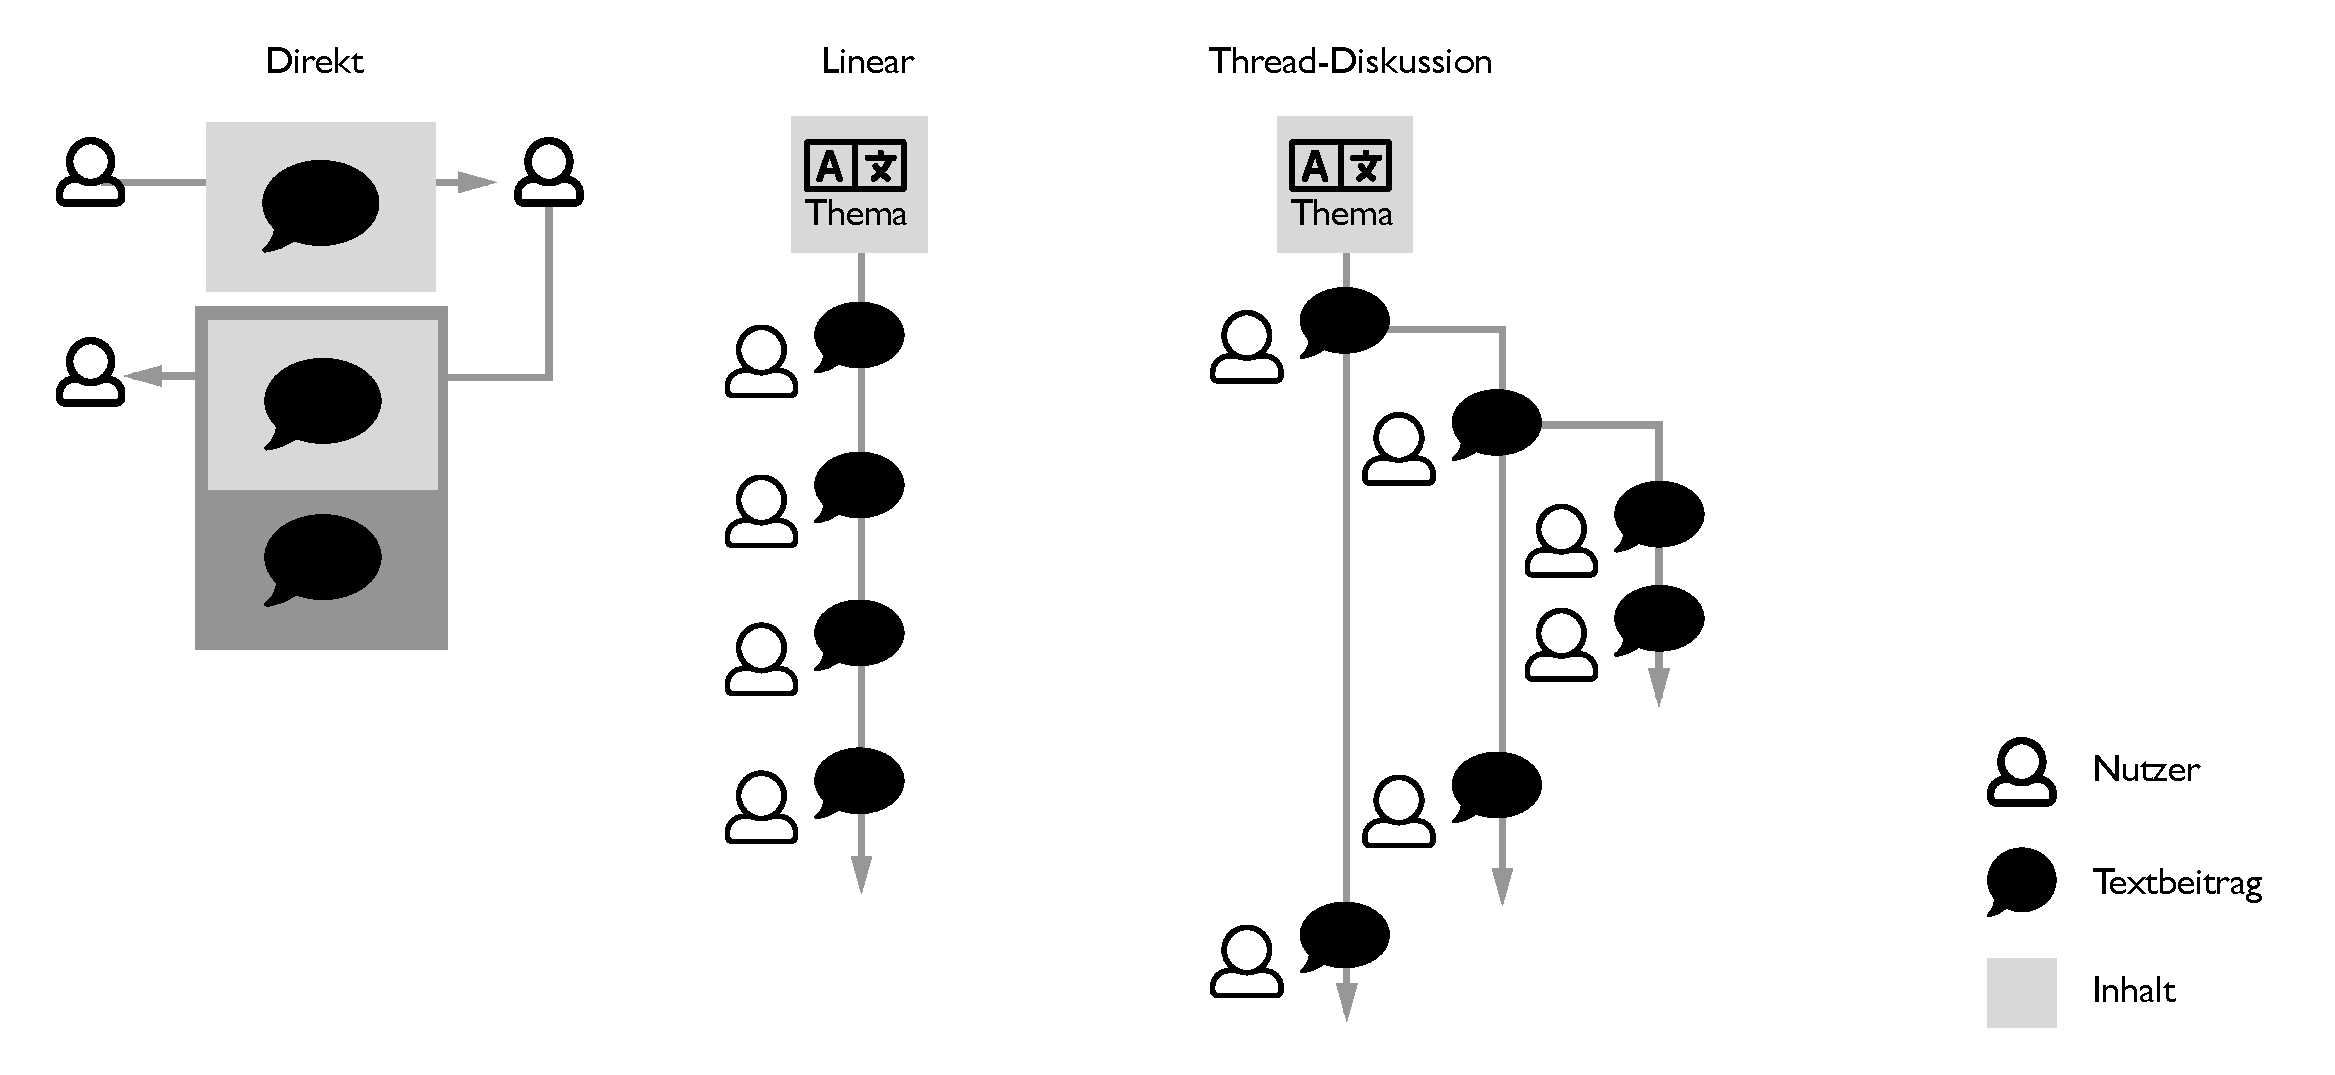
\includegraphics[width=\textwidth]{figures/kommentar_illustration.pdf}    
\end{figure*}  
% \begin{labeling}{whats}
%   \item [post (Verb: posting)] Textbeitrag eines Nutzers.
%   \item [Kommentar] Ein Textbeitrag im Bezug auf einen Post.
%   \item [Thread] Eine Sammlung von Kommentaren
% \end{labeling}

\section{Direkt}
In der direkten Kommunikation senden Nutzer \user Nachrichten \comment direkt. 
Der Kontext einer Nachricht 
besteht dann zwischen \mbox{\(\text{\user} \mapsto \text{\comment} \mapsto \text{\user} \)}.
Chat und Email sind Beispiele für diese Form.

\section{Linear}
Auf Online-News-Webseiten, wie zum Beispiel \url{spiegel.de}, können Nutzer Kommentare 
zu Artikeln schreiben (Relation \(\text{\lang} \mapsto [\maththree{\comment} \dots]\)).
Die Kommentare können dann chronologisch sortiert werden. 

Bei vielen Nutzer wird in dieser Form ein Problem deutlich: 
Ein Text hat immer auch eine semantische Komponente (z.B. unterschiedliche Aspekte eines Themas).
Gibt es ein \ca{Thema A} und eine \cb{Thema B}, dann müssen Nutzer dies im Text schreiben.
\(\text{\lang} \mapsto
[\text{\ca{\comment}}_1, 
\text{\cb{\comment}}_2,
\text{\ca{\comment}}_3, \dots]\) 

Bulleltin Boards versuchen dieses Problem zu lösen in dem Nutzer andere Nachrichten als Zitat in neue Nachrichten einbauen können. 


\section{Thread-Diskussion}
\label{sec:Threaded}
Ein Thread-basiertes Komentarsystem erlaubt es Nutzern nicht nur Inhalte zu kommentiern (\(\text{\lang} \mapsto \text{\comment}_i\) )
,sondern auch ein anderen Kommentar \(\text{\comment} \mapsto [\maththree{\comment} \dots]\).
Dadurch entsteht eine Baumstruktur. Wie diese Struktur in der Diskussion genutzt wird, hängt von 
den Konventionen der Plattform ab. Diese werden auch stark durch das Nutzerinterface einer
Website geprägt.
Generell kann in Thread-Diskussion auf zwei Arten \cb{geantwortet} werden.
Sequentiell  \(\text{\comment} \mapsto
[\text{\comment}, 
\text{\cb{\comment}}]\) 
oder direkt \(\text{\comment} \mapsto
[\text{\comment} \mapsto [ 
\text{\cb{\comment}}]]\)
% \begin{marginfigure}
%   
\includegraphics[width=\textwidth]{figures/facebook-com-tagesschau.png}
%   \caption{\url{https://www.facebook.com/tagesschau/posts/10155847201279407}}
% \end{marginfigure}


% - Anpassung der Representationen an die Aufgabe (NormanThingsThatMake1994)
%   - 
% - Darstellungsformen
% - Begriffserklärung
%   - Plattform
%     - Technische Lösung zum Publizieren von Beiträgen
%     - Verwaltet alle Aspekte der Community (Identitäten, Zensur)
%   - Beitrag (Content) 
%   - Community 
%     - Menge an Nutzern
%     - In der Anfangsphase des Internets 
%   - Thread
%     - dt. Faden
%     - Chronologische Folge von Beträgen
%   - Textbeitrag

\subsection{Sichtbar und Interaktionen}
\label{sec:sichtbarkeit}
Thread-Diskussionen haben aber auch Probleme.
Eine sehr große Menge an Subkommentaren kann Kommentare,
die direkt auf das Thema antworten, außerhalb des Sichtbereichs 
drängen (Abbildung \ref{ref:viewport}).

Kommentare die zuerst gesehen werden erhalten mehr Aufmerksamkeit.
Dies kann wiederum die Sortierung der Kommentare beeinflussen (siehe Abschnitt \nameref{sec:reddit}).
% Dadurch kann das 

\begin{figure}
  \caption{  
    Nur sehr wenige Kommentare haben viele Upvotes
  }  
    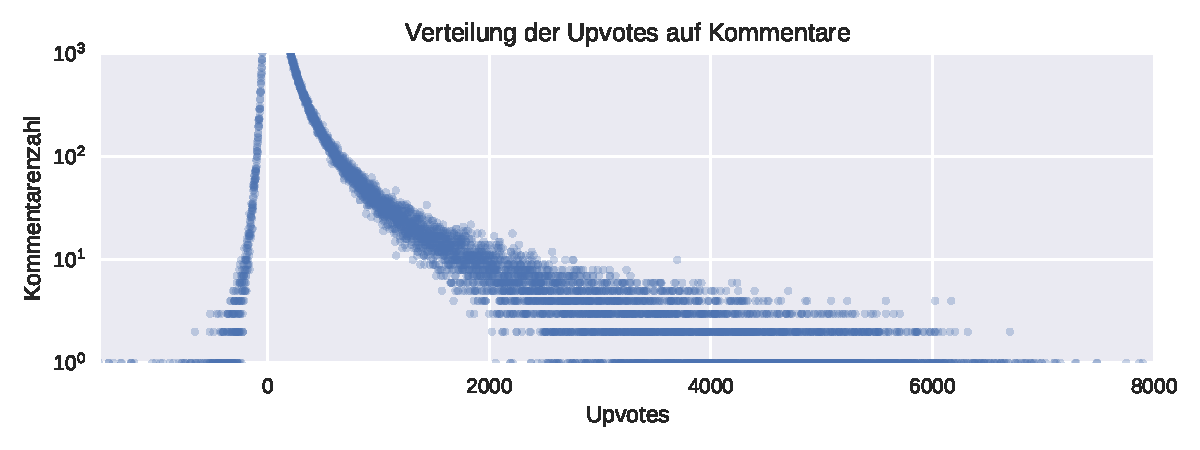
\includegraphics[width=\textwidth]{figures/upvote_distribution2016_1.pdf}
    \label{ref:viewport}
  \end{figure}     

\begin{marginfigure}
  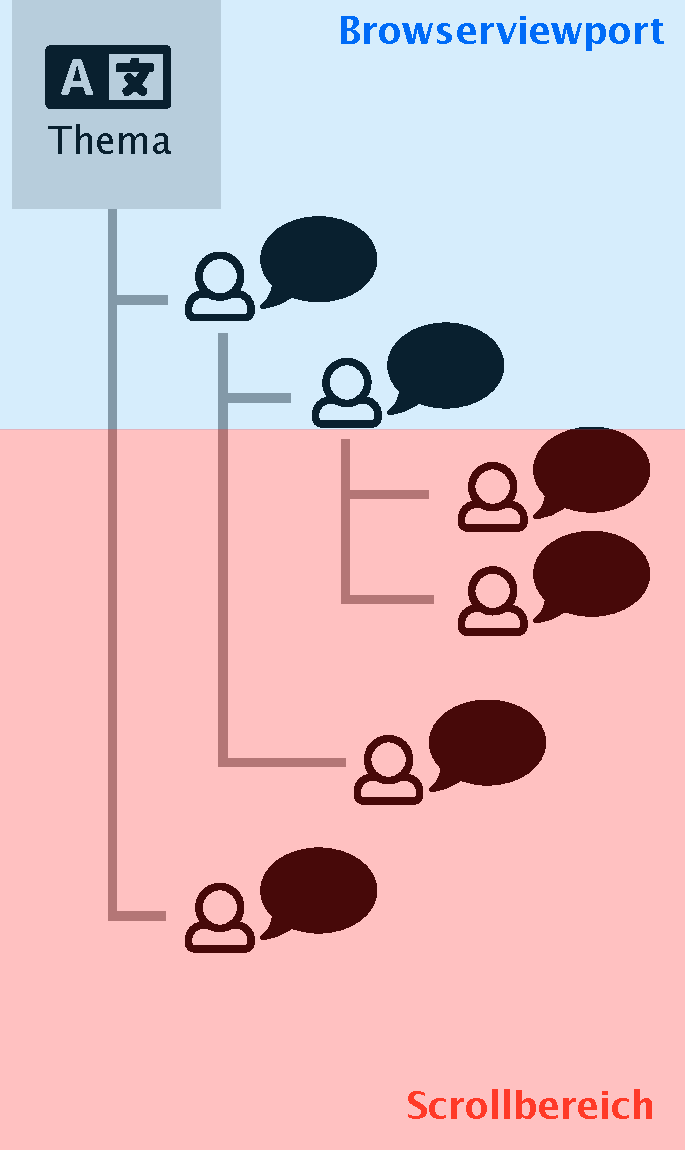
\includegraphics[width=\textwidth]{figures/browser_cutoff.pdf}
  \caption{Je mehr Unterkommentare das erste Kommentar hat, desto weniger sichtbar sind andere Root-Kommentare}
\end{marginfigure}


\chapter{Visualisierung}
%Im praktischen Teil der Arbeit soll eine interaktive Visualisierung enstehen,


Die Umsetzung einer Visualisierung umfasst nicht nur die Bereiche Statistik und Grafikdesign,
inzwischen spielt Informatik eine Hauptrolle im Informationsdesign.
\citeauthor{FryComputationalinformationdesign2004} \cite{FryComputationalinformationdesign2004}
bezeichnet diese Mischung von Fachbereichen als  \textbf{``Computional Information Design''}. 
Er definiert auch einen Prozess (Abbildung \ref{fig:fry-steps}) um die Vorgehensweise im Informationsdesign zu verdeutlichen. 
Die Beschreibung der Umsetzung dieser Arbeit orientiert sich an diesen Schritten.
\begin{figure}
  \label{fig:fry-steps}
  \caption{ Arbeitschritte \cite[164]{FryComputationalinformationdesign2004}}  
    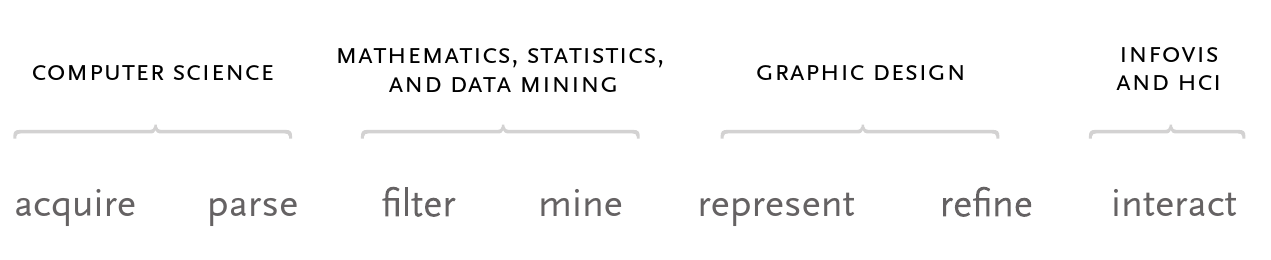
\includegraphics[width=\textwidth]{figures/fry_steps.png} 
\end{figure} 


\section{Datenbeschaffung (acquire)}
Es sind viele aufbereitete Datensets verfügbar die Postings von Usern enthalten und es 
gibt noch mehr potentielle Datenquellen. 
Social Media Plattformen stellen Programmierschnittstellen (APIs) bereit auf denen Daten direkt,
meist im JSON-Format, abgerufen werden können. 
Jedoch sind diese für die Entwicklung von Endanwendungen gedacht.
Das Herunterladen größer Mengen an Beiträgen ist unerwünscht, limitiert und unterliegt
rechtlichen Auflagen. Meistens ist nur eine nichtkommerziele Nutzung erlaubt.

Im Abschnitt \nameref{sec:sichtbarkeit} wurden die Probleme genannt, die bei einer Diskussion mit sehr vielen
beteiligten und vielen Kommentaren auftreten. 
Das Datenset für die Visualisierung sollte deshalb auch sehr umfangreiche Diskussion enthalten.
Beiträge sollten auch im Thread-Format vorliegen (siehe \nameref{sec:Threaded}).

Ein Datenset, dass diesen Anforderungen entspricht, ist das von \citeauthor{BaumgartnerRedditData2017} erstellte \emph{reddit}-Datenset \cite{BaumgartnerRedditData2017}.

\subsection{reddit.com}
\label{sec:reddit}
Die Webseite \emph{reddit.com} wird von 6\% der U.S. Amerikanischen Internetnutzern genutzt\cite{DugganOnlineAdultsare2013} . Reddit ist ein ``link aggregator'' (dt. Linksammler).
Diese Art von Social Media Plattformen bietet Nutzern zwei Hauptfunktionen:
Nutzer können URLs ``posten'' und diese bewerten. Jede URL kann kommentiert werden.
Zusätzlich ist es möglich auf Posts und Kommentare positiv oder negativ zu bewerten.
Diese Interaktion wird Voting genannt und ermöglicht Kommentare nach einer zusätzlichen Dimension zu 
ordnen. In den Verhaltensregeln für reddit (die ``reddiquette'' \cite{redditreddiquette}) wird \emph{voting} wie folgt beschrieben:

\begin{quote}
  \textbf{Vote.} If you think something contributes to conversation, upvote it. If you think it does not contribute to the subreddit it is posted in or is off-topic in a particular community, downvote it.
\end{quote}

Standardmäßig wird die Beziehung \(\text{\comment} \mapsto [\maththree{\comment} \dots]\) nicht
chronologisch sortiert, sondern nach einem Maß, dass aus den ``up'' und ``down'' Wahlen erechnet
wird \cite{MillerHowNotSort2009}.

Reddit bietet eine offizielle Programmierschnittstelle (\textbf{API}) an, aber diese unterliegt bestimmten \textbf{Begrenzungen}
ähnlich denen anderer Plattform. Die exakte Menge an up/down Wahlen ist geheim und es wird nur ein Wert (``ups'') ausgeben.
Die API ist auf ein bestimmtes Featureset begrenzt. Eine Suche nach Einreichungen mit einer hohen Kommentaranzahl
ist nicht möglich.

Deswegen verwende ich ein ``offline'' Datensatz der Reddit-Kommentare\cite{BaumgartnerRedditData2017}.
Der Datensatz beinhaltet alle Reddit-Kommentare und ist unterteilt Monate. 
Abbildung \ref{fig:monthly} zeigt, dass der Datensatz aktuell mehr als 3500 Millionen Kommentare enthält.


\begin{figure}
  \label{fig:monthly}
  \caption{Kommentaranzahl in \cite{BaumgartnerRedditData2017}}  
    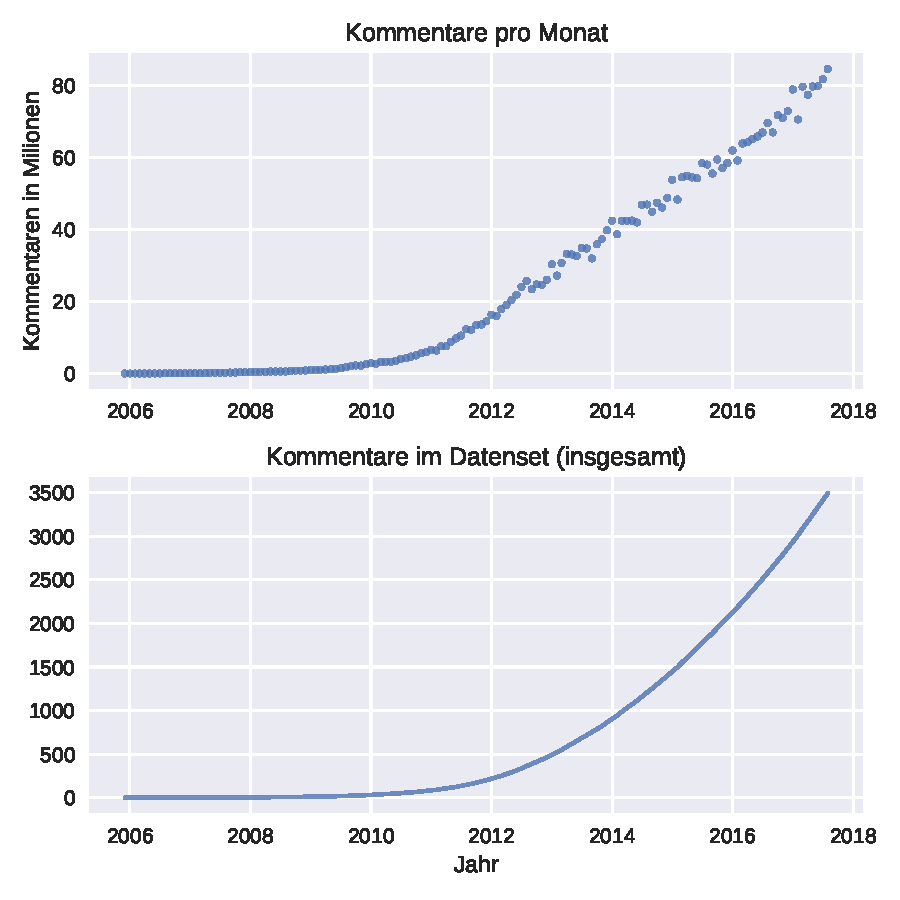
\includegraphics[width=\textwidth]{figures/monthlyCount.pdf}  
  \end{figure}



\section{Datenformat (parse)}
Der Datensatz enthält  Kommentare im JSON-Format, die jeweils durch Zeilenumbrüche getrennt sind. 
Ein Beispiel-Datensatz ist hier aufgelistet:

\begin{lstlisting}[language=json,firstnumber=1,label=codejson]
  {'author': 'RoboChrist',
  'author_flair_css_class': None,
  'author_flair_text': None,
  'body': 'There\'s "s ...',
  'controversiality': 0,
  'created_utc': 1452097977,
  'distinguished': None,
  'edited': False,
  'gilded': 0,
  'id': 'cyo5nvp',
  'link_id': 't3_3zpp3w',
  'parent_id': 't1_cyo4in3',
  'retrieved_on': 1454317397,
  'score': 158,
  'stickied': False,
  'subreddit': 'dataisbeautiful',
  'subreddit_id': 't5_2tk95',
  'ups': 158}
\end{lstlisting}

Aufgrund der hohen Speicherplatzanforderung habe ich mich zuerst nur auf Daten aus dem Jahr 2016 beschränkt. Die Kommentare für 2016 sind allein 80 GB groß.
Für die Verarbeitung der Dateien habe ich das Pythonframework Dask \cite{RocklindaskParallelcomputing2017} verwendet.
Die Dask-API erstellt programmatisch ein Ausführungsbaum (``compute graph''),
der dann parallel auf den Zeilen des Datensatzes ausgeführt werden kann.
Mit dem folgenden Code-Beispiel wurde die durschnittliche Länge der Kommentare gemmessen: 

\begin{lstlisting}[language=python]
  jsons  = lines.map(json.loads)
  length = jsons.map(lambda data: len(data['body']))
  freq   = length.frequencies()
  result = client.compute(freq).gather(future)
\end{lstlisting}

\begin{figure}
\caption{  Ein reddit-Kommentar hat eine maximale Länge von 10000 Zeichen.
Für entfernte und gelöschte Kommentare werden über die Zeichenketten \jc{[removed]}
und \jc{[deleted]} dargestellt.
}  
  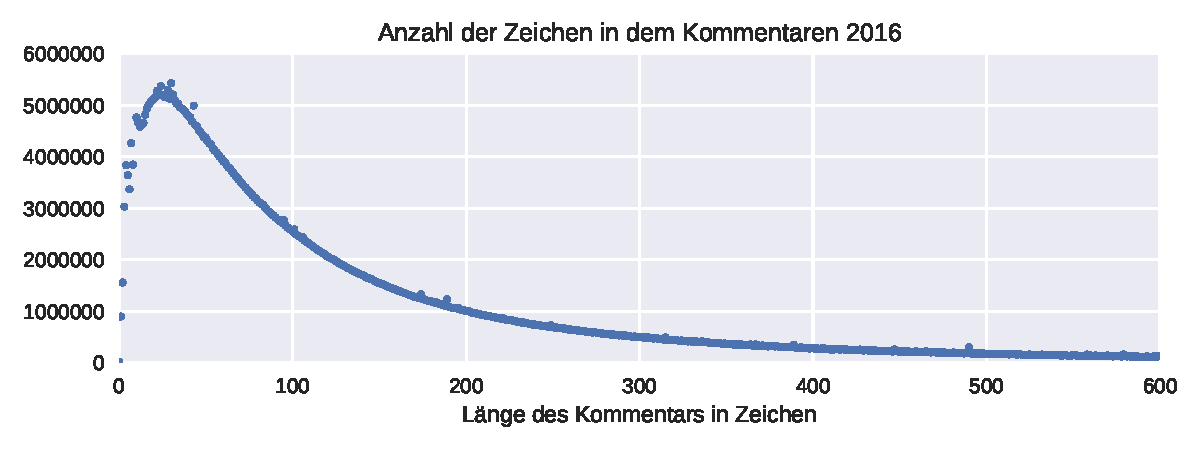
\includegraphics[width=\textwidth]{figures/comment_length_frequencies2016.pdf}  
\end{figure}

Dask ist ideal für die Stapelverarbeitung großer Datenmengen, aber für eine Visualisierung von Thread-Diskussionen ist nicht immer nötig den gesamten Datensatz zu filtern.

\subsection{Datenbank}
Die Datenbank von \emph{reddit} selbst speichert alle Daten auch als {key/value}-Paare ab \cite{EdbergScalingRedditMillion2013}. 
Reddit-Entwickler haben es dadurch leichter neue Features zu implementieren.
Normalerweise müsste das Datenbankschema angepasst werden und das ist nicht trivial.
Deswegen habe ich die gleiche Schemaart für die Datenbank der Visualisierung verwendet. 
Als Datenbank verwende ich die relationale Datenbank Postgres.
Die Tabelle der Kommentare hat nur zwei Reihen: \texttt{id} und \texttt{data}.
Trotzdem kann man mit dem Datentyp \texttt{jsonb} direkt auf die JSON-Elemente zugreifen.

Die folgende Suchanfrage findet Kommentare die einem Thread angehören und 
braucht auf dem Datensatz von 62 Millionen Kommentaren 1:22 Minuten. 

\begin{lstlisting}[language=sql,firstnumber=1]
  select data from comments 
  where 
    data->>'link_id' = 't3_42n6x9' 
\end{lstlisting}

Für Anfrage wie diese wird deswegen ein Index auf das Feld \texttt{link\char`_id} erstellt. 
Die gleiche Anfrage braucht mit Index nur noch 2.8s. 


\section{filter}
Jeder Kommentar in der Datenbank hat ein Feld \texttt{parent\_id},
mit der die Relation zum Elternknoten hergestellt wird.
So einsteht am Ende eine Baumstruktur, deren Wurzel immer eine reddit-``submissions'' steht.
\marginnote{reddit-``submissions'' sind Elemente aus einer Überschrift+URL oder einer Überschrift+Text  }

Es ist aber auch möglich die Relation \relto{\comment}{\comment}
als Relation zwischen Usern zu verstehen \relto{\user(\comment)}{\user(\comment)}
\begin{figure}
  \caption{  
    Graph der Interaktionen in einem Thread: 
    Jeder Knoten stellt einen Author dar. 
    Authoren die auf ein Kommentar geantworted haben 
    sind durch eine Kante verbunden.  
  }  
    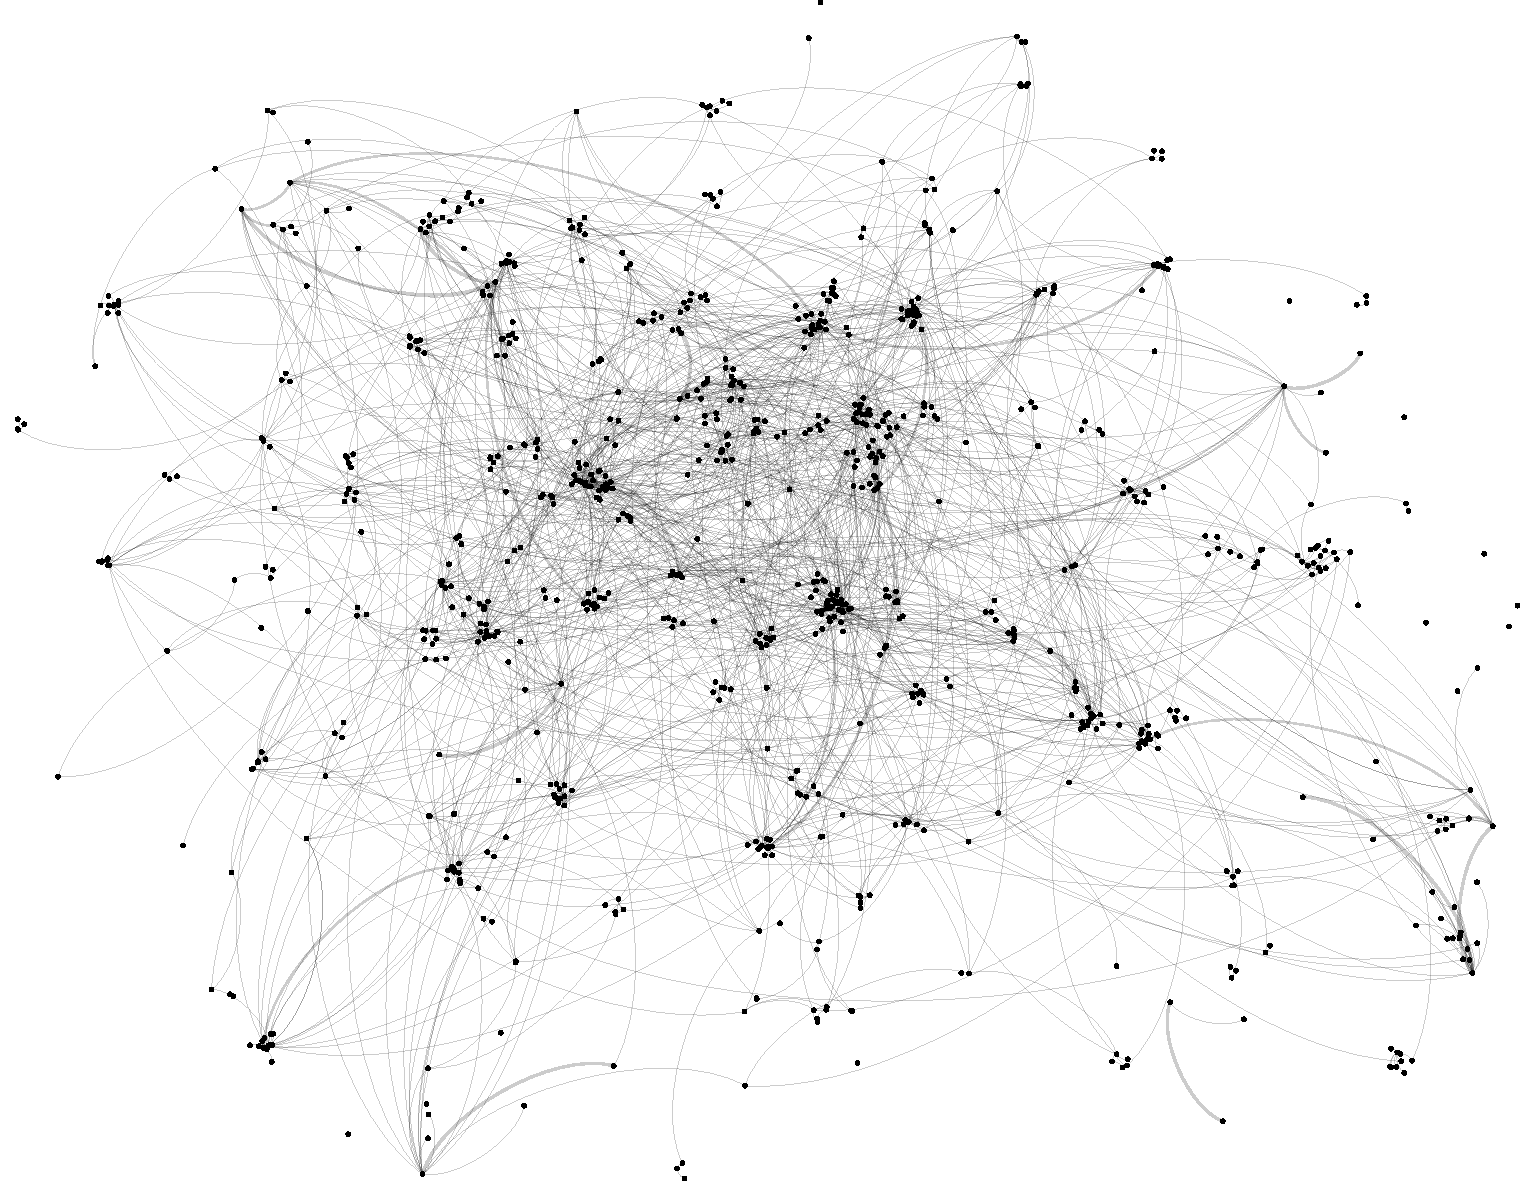
\includegraphics[width=\textwidth]{figures/comment_graph_interactions.pdf}
    \label{fig:interactions}
\end{figure} 

Abbildung \ref{fig:interactions} zeigt einen Graphen, der aus den diesen Relationen gebiltet wurde.
Ich habe den Graphen nur Testweise erstellt, um zu sehen, ob sich die Visualisierung lohnt.
Jedoch haben die getesteten Graphlayout-Algorithmen kein zufriedenstellendes Ergebnis geliefert.

\section{mine}
Populäre Reddit-Diskussionen erhalten bis zu 30000 Kommentare oder mehr,
aber nur wenige haben ereichen eine solches Ausmaß, wie die Abbildung \ref{fig:bigcomments} zeigt. 


\begin{marginfigure}
  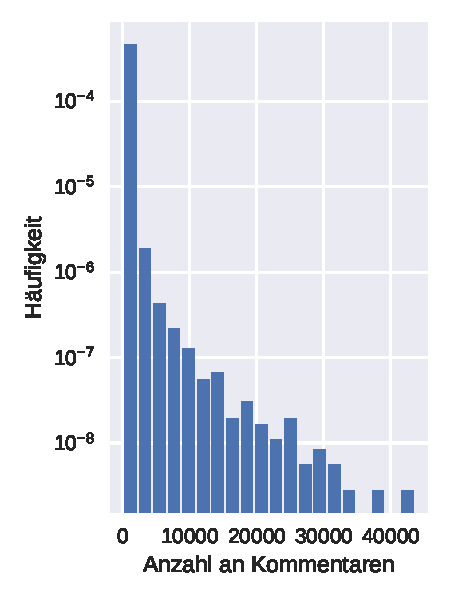
\includegraphics[width=\textwidth]{figures/biggest_threads_2017_1.pdf}
  \caption{Die Menge der Kommentare ist logarithmisch auf die Einreichungen verteilt}
  \label{fig:bigcomments}
\end{marginfigure}



\section{Repräsentationen}

Die Darstellung der Kommentartexte alleine übersteigt schnell die Größe eines HD-Bildschirms:
Bei durchschnittlich 177 Zeichen pro Kommentar und z.B. 4000 Kommentaren müsste man 
708000 Zeichen darstellen. Die Menge an Zeichen pro Textzeile ist auf etwa 80 begrenzt,
da Texte sonst nur schwer lesbar sind. Mit einer Zeilenhöhe von etwa 22 Pixel
sind allein für den Text fast 200000 Pixel nötig.

Um trotzdem den Kontext eines Kommentares zu visualisieren habe ich ein Overview+Detail 
Schema verwendet. Ein overview+detail Interface stellt Kontext und Detail gleichzeit, aber 
räumlich getrennt dar \cite{CockburnReviewOverviewDetail2009}.
Das Detail ist der Text in lesbarer Auflösung.
Der Kontext ist die Datenstruktur des Kommentartthreads ohne Text.

\begin{marginfigure}
  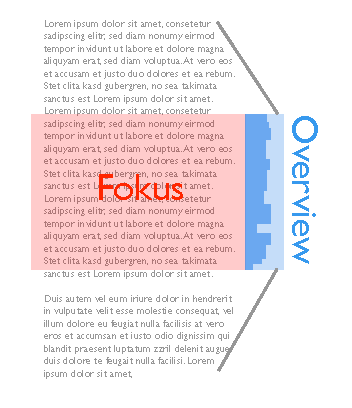
\includegraphics[width=\textwidth]{figures/Kontext.pdf}
  \caption{\cb{fokus} + \ca{overview} = Viewport}
  \label{figcontext}
\end{marginfigure}

Diese Datenstruktur ist ein Baum, aber die klassische Darstellung von Bäumen 
hat kein gutes ``data/ink''-Verhältniss \cite{TufteVisualDisplayQuantitative2009}.
Zum anderen, ist die Darstellung optisch gesehen nicht sehr simpel
(Die rote Linie in Abbildung (a) soll die ``unruhige'' optische Linie zeigen).
Der ``icicle plot'' ist für die Darstellung von Clusterungen gedacht,
deswegen ist die Höhe eines Knotens durch die Summe der Höhen seiner Kinder bestimmt.

Für die Darstellung von Kommentaren zeichne ich aber alle Knoten mit gleicher Höhe 

\begin{figure*}
  \centering
  \begin{subfigure}[b]{0.3\textwidth}
    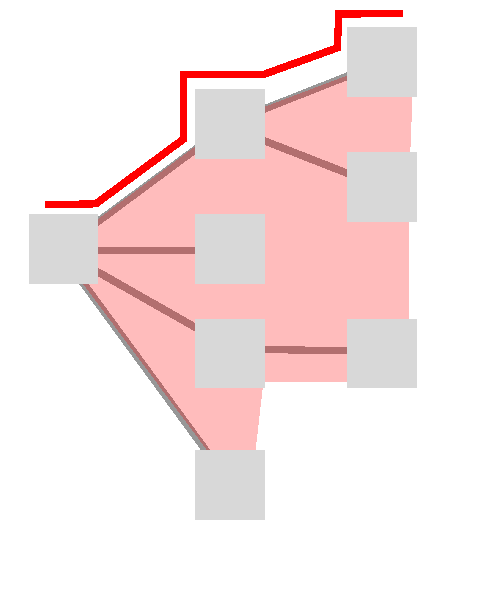
\includegraphics[width=\textwidth]{figures/tree_display1.pdf} 
    \caption{ Klassisch }  
    \label{fig:treesa}   
  \end{subfigure}
  \begin{subfigure}[b]{0.3\textwidth}
    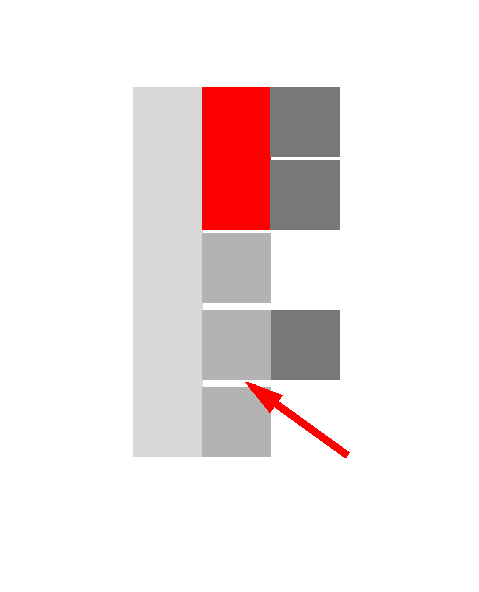
\includegraphics[width=\textwidth]{figures/tree_display2.pdf} 
    \caption{ icicle plot, der \cb{Knoten} überspannt die Unterknoten}  
    \label{fig:treesb}   
  \end{subfigure}
  \begin{subfigure}[b]{0.3\textwidth}
    
\includegraphics[width=\textwidth]{figures/tree_display3.pdf} 
    \caption{ ``Icicle'' Baum, uniforme Knoten}  
    \label{fig:treesc}   
  \end{subfigure}
  \caption{Baumlayoutmethoden}
  \label{fig:trees}
\end{figure*}

\section{refine}
Die Höhe des \emph{icicle plots} wird an die Höhe des Browser-Viewports angepasst.
Bei einer sehr hohen Anzahl an Knoten kann es vorkommen, dass die Höhe eines Knotens kleiner wird als 1px. 
Die Visualisierung wird dann durch das \emph{anti aliasing} des Browsers heller als gewollt (siehe Abbildung a).

\begin{figure*}
  \centering
  \begin{subfigure}[b]{0.3\textwidth}
    
\includegraphics[width=\textwidth]{figures/treegraphs/midcount.png}
    \caption{Normal}
    \label{fig:map:mid}
  \end{subfigure}
  \begin{subfigure}[b]{0.3\textwidth}
    
\includegraphics[width=\textwidth]{figures/treegraphs/midcount_minheight.png}
    \caption{Höhe min. 1px}
    \label{fig:map:midmin}
  \end{subfigure}
  \begin{subfigure}[b]{0.3\textwidth}
    
\includegraphics[width=\textwidth]{figures/treegraphs/midcount_minheight_rounded.png}
    \caption{y Position gerundet}
    \label{fig:map:midminround}
  \end{subfigure}
  \caption{Ausgabe des Layouts auf dem HTML-Canvas}
\end{figure*}

Durch eine Mindesthöhe wird das verhindert. Des weiteren wird die y-Position der Knoten
auf ganzzahlige Werte gerundet, damit die Kanten schärfer dargestellt werden. 

\section{interact}
\begin{figure*}
  \caption{ Workflow zur Erarbeitung der Visualisierungen }  
    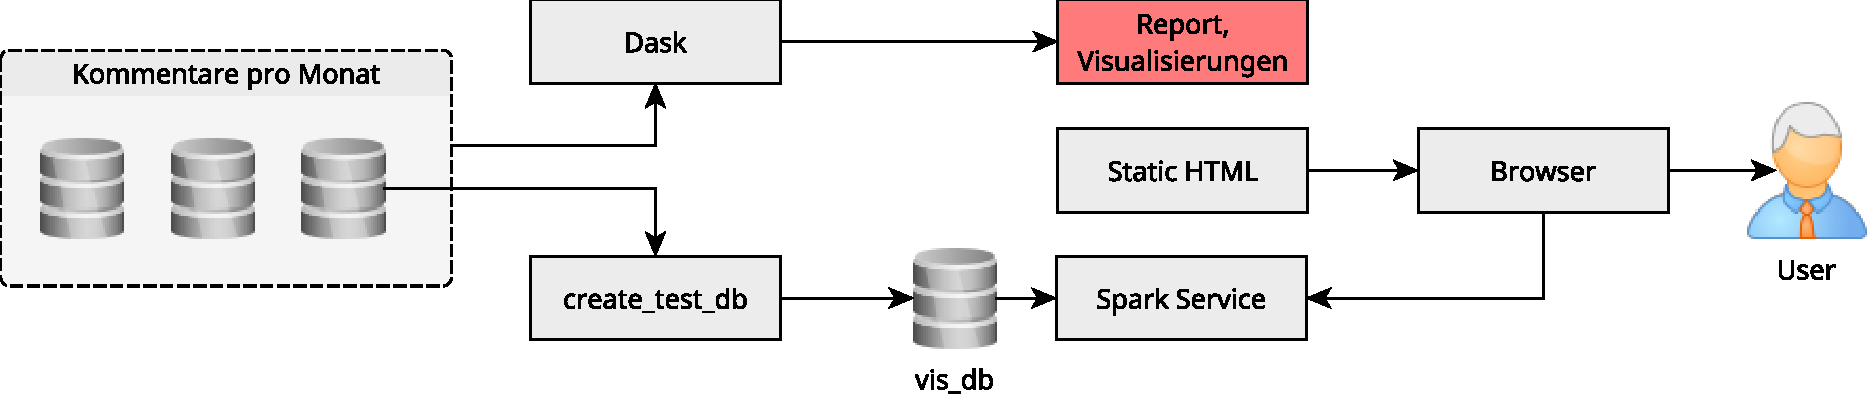
\includegraphics[width=\textwidth]{figures/workflow.pdf} 
    \label{workflow}
\end{figure*} 
Die Abbildung \ref{workflow} zeigt alle Elemente der Visualisierungs-Anwenung.
Die Visualisierung selbst wurde mittels der JavaScript Bibliothek D3.js umgesetzt \cite{BostockD3js2011}.

Der Source-Code der Visualisierung, geschrieben in ECMAScript 6,  
wird zusammen mit allen Abhängigkeiten in eine Scriptdatei transpiliert.
 
Vom Browser des Nutzers wird die REST-API des Backends abgefragt. 
Das Backend führt dann den SQL-Befehl aus und liefert die Daten in Form von JSON an den Browser.
Aufgrund der hohen Anzahl von Elementen wird der Kommentarbaum im Browser in einem Canvas-Element
gezeichnet und nicht in Form von SVG-Elementen dargestellt. 

\section{Zusammenfassung}
Die vorgestellte Visualisierung zeigt eine Möglichkeit die Struktur von Thread-Diskussionen sehr 
kompakt darzustellen. 
Die größten Schwierigkeiten lagen im Bereich der Anwendungsentwicklung und Koordination
der heterogenen Webtechnologien.  

\begin{figure*}
  \caption{ Screenshot der Endanwendung}  
  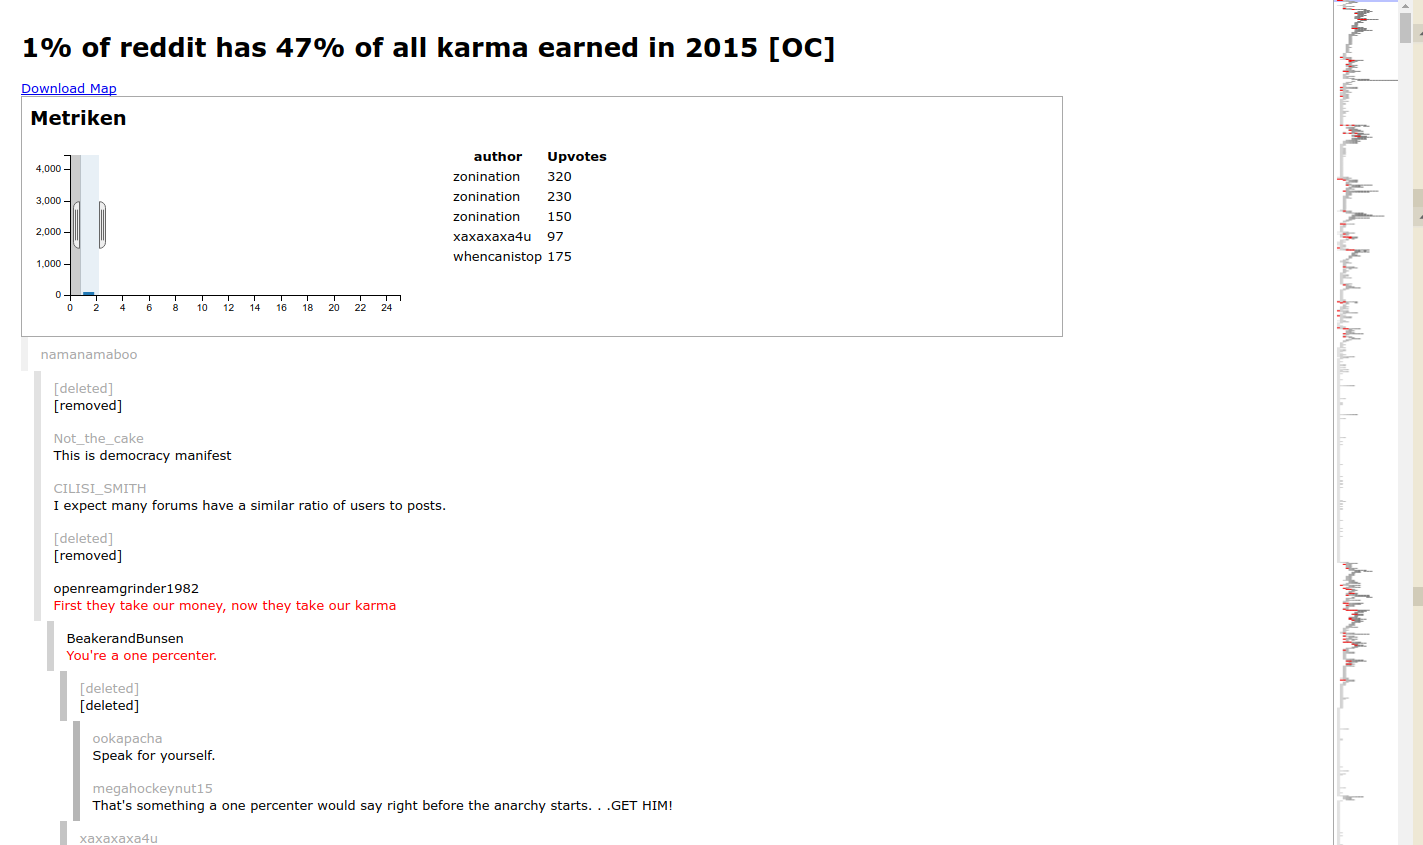
\includegraphics[width=\textwidth]{figures/app_screen.png} 
  \label{screen}
\end{figure*} 


\printbibliography
\end{document}